%------------------------------------------------

\begin{fullwidth}
Publication typically involves multiple iterations of manuscript,
code, and data files, with inputs from multiple collaborators.
This process can quickly become unwieldy.
It is in nobody's interest for a skilled and busy researcher
to spend days re-numbering references (and it can take days)
when a small amount of up-front effort can automate the task.
Similarly, simultaneous collaboration should not involve
the repetitive and error-prone task of manually resolving
sets of tracked-changes documents with conflicting edits.
Furthermore, for most research projects,
completing a manuscript is not the end of the task.
Academic journals often require a ``reproducibility package''
which contains the code and materials used to create the results.
These represent an intellectual contribution in their own right,
because they enable others to learn from your process
and better understand the results you have obtained.
Holding code and data to the same standards as written work
is a new practice for many researchers.

In this chapter, we suggest tools and workflows for efficiently managing collaboration
and ensuring reproducibility.
First, we discuss how to use dynamic documents to collaborate on technical writing.
Second, we provide guidelines for preparing a functioning and informative reproducibility package.
If you have organized your analytical process
according to the general principles outlined in earlier chapters,
preparing to publish materials will not require
substantial reorganization of the work you have already done.
Hence, publication is the conclusion of the system
of transparent, reproducible, and credible research we introduced
from the very first chapter of this book.
We include specific guidance on publishing both code and data files,
noting that these can be a significant contribution in addition to written results.
In all cases, we note that technology is rapidly evolving
and that specific tools noted here may not remain cutting-edge,
but the core principles involved in publication and transparency will endure.
\end{fullwidth}

%------------------------------------------------

\section{Preparing written documents for publication}

% collaborating is easier with dynamic documents
Development research is increasingly a collaborative effort.
This reflects changes in the economics discipline overall:
the number of sole-authored papers is decreasing,
and the majority of recent papers in top journals have three or more
authors.\sidenote{\url{https://voxeu.org/article/growth-multi-authored-journal-articles-economics}}
As a consequence, manuscripts typically pass back and forth between several writers
before they are ready for publication.
Just as with the preparation of analytical outputs,
effective collaboration requires the adoption of tools and practices
that enable version control and simultaneous contribution.
As we outlined in the previous chapter,
\textbf{dynamic documents} are a way to simplify writing workflows:
updates to analytical outputs that appear in these documents, such as tables and figures,
can be passed in to the final output with a single process,
rather than copy-and-pasted or otherwise handled individually.
Managing the writing process in this way
improves organization and reduces error,
such that there is no risk of materials being compiled
with out-of-date results, or of completed work being lost or redundant.

\begin{fullwidth}
	\begin{figure}
		\centering
		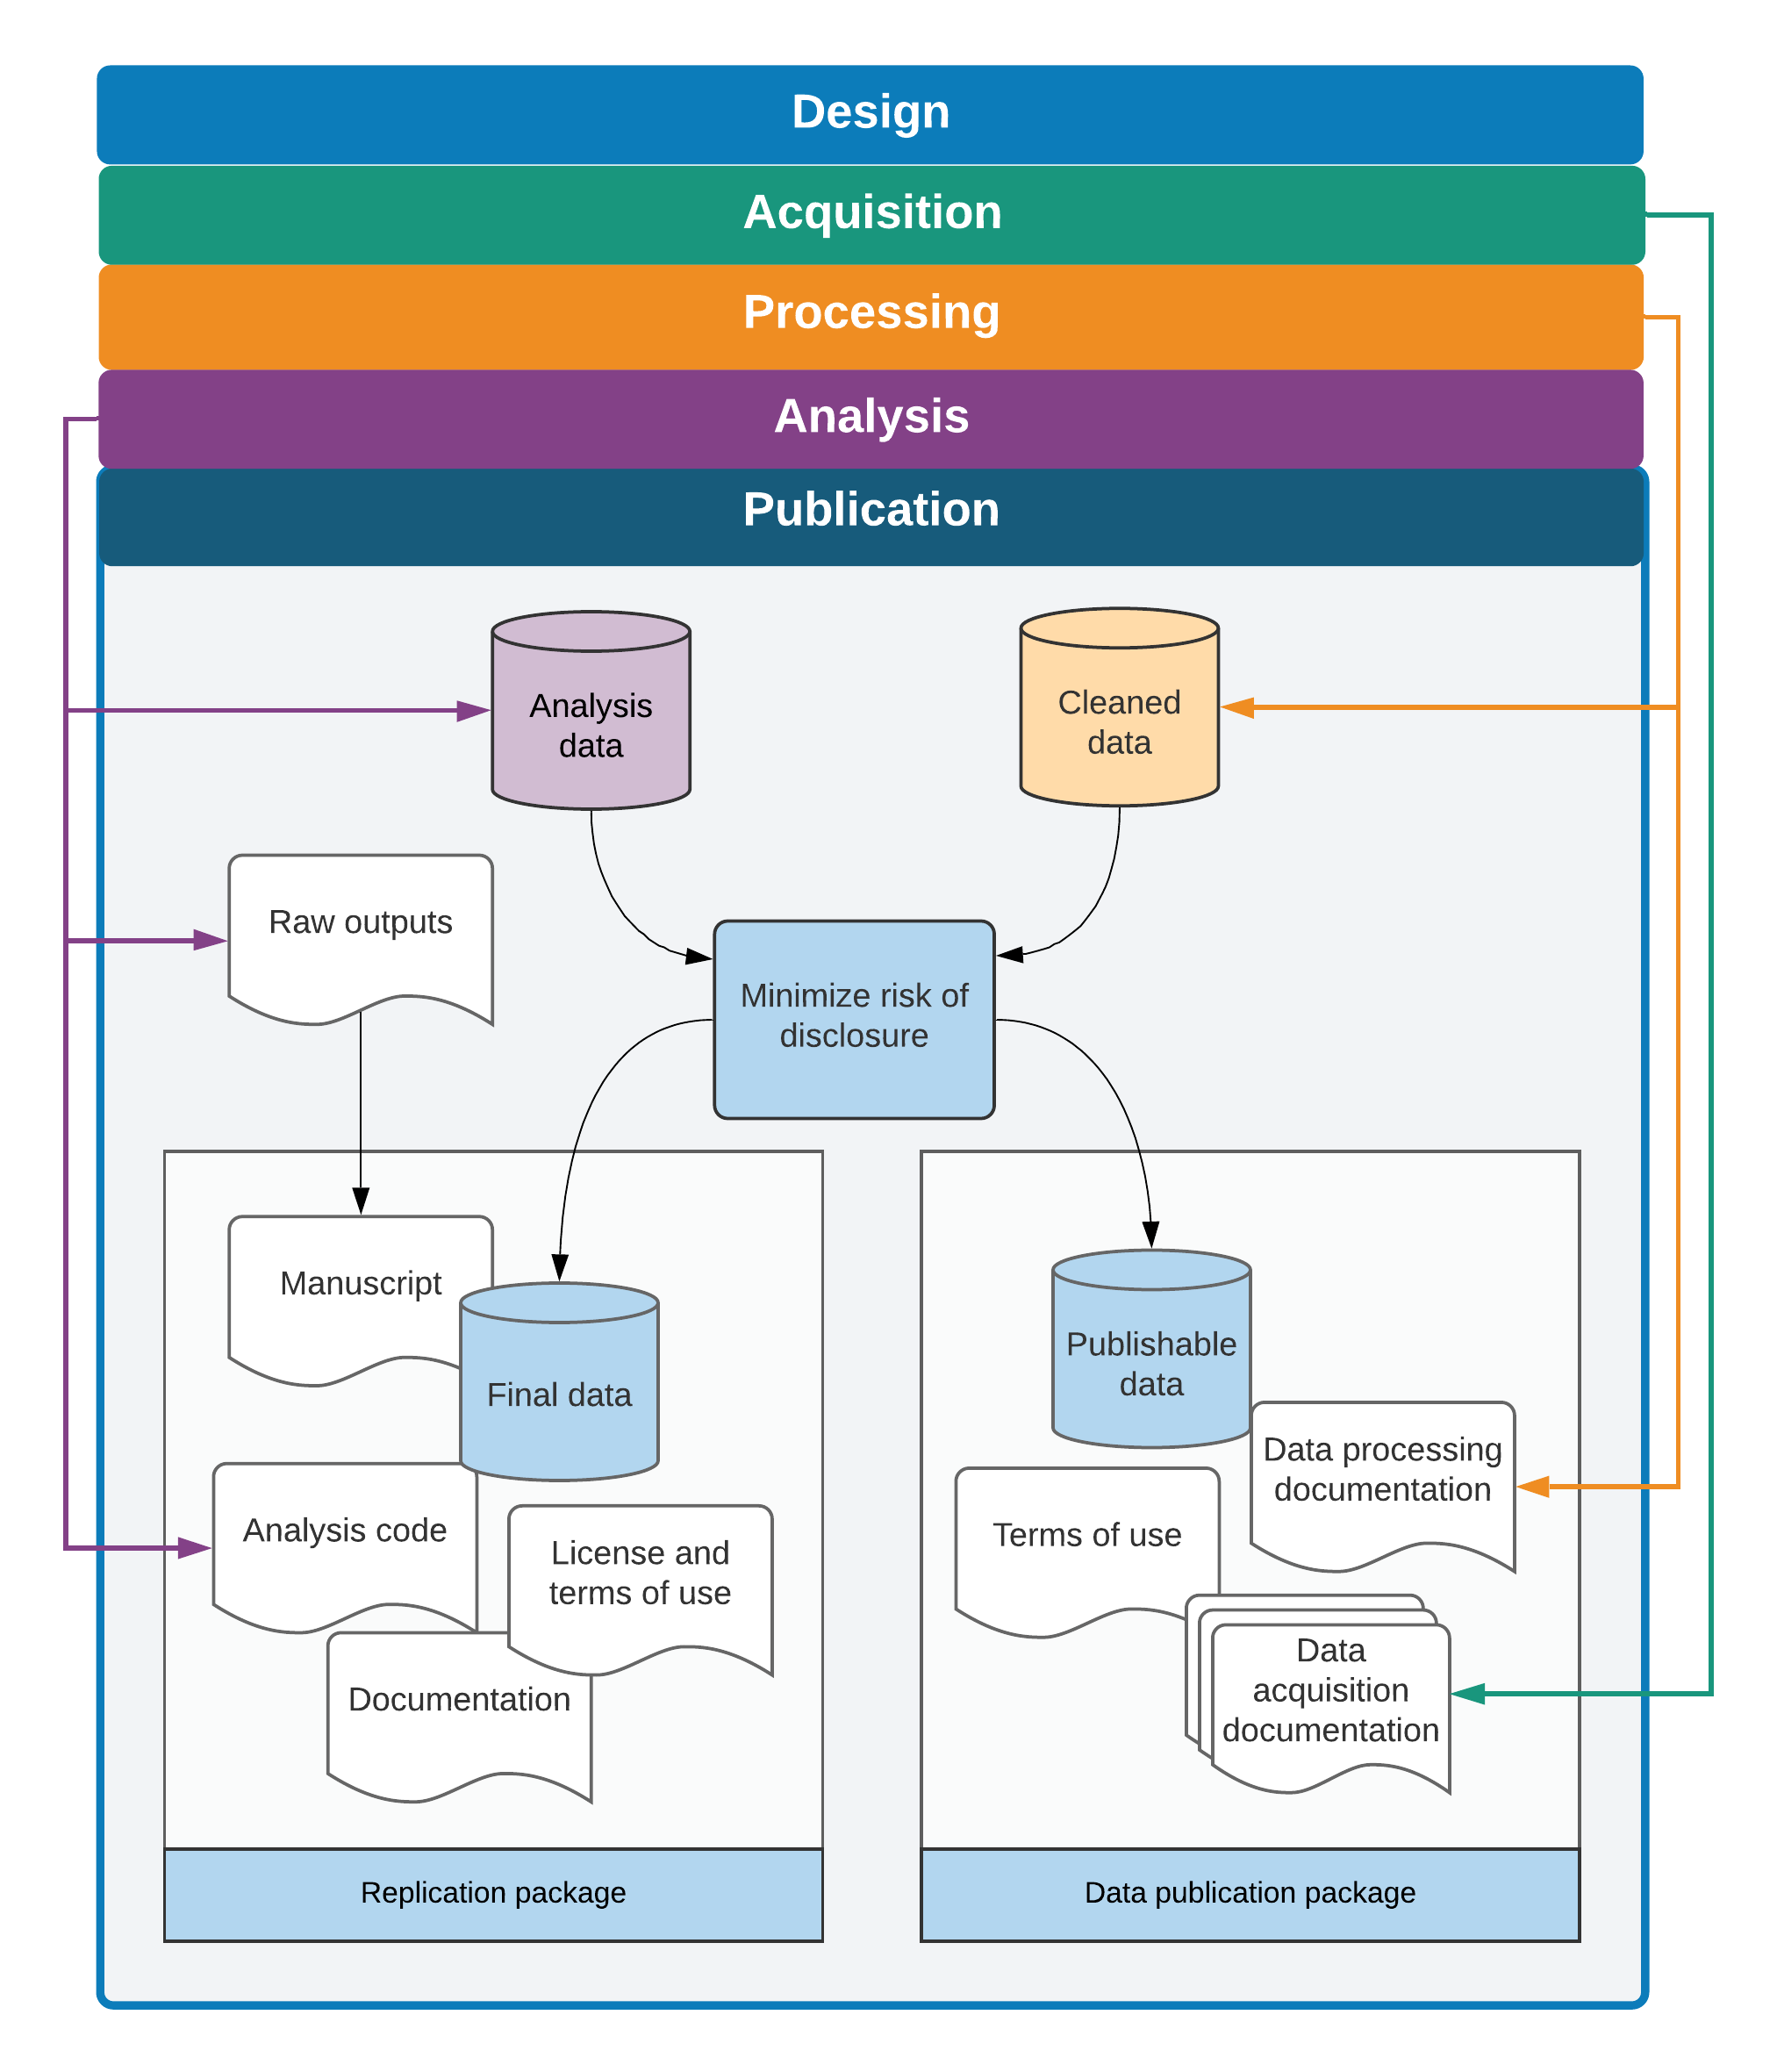
\includegraphics[width=1.6\linewidth]{diagrams/Publication}
		\caption{}
		\label{fig:intro}
	\end{figure}
\end{fullwidth}

\subsection{Preparing manuscripts as {\LaTeX} documents}

% what exactly is a dynamic document
As we discussed in Chapter 6, the most widely used software
for dynamically managing academic manuscripts is {\LaTeX} (pronounced ``lah-tek'').
\index{\LaTeX}
It requires explicitly encoded references to the latest versions of all outputs.
This is not possible by default in Microsoft Word.
There, you have to copy and paste each object
whenever tables, graphs, or other inputs are updated.
As time goes on, it becomes more and more likely
that a mistake will be made or something will be missed.
In {\LaTeX}, instead of writing in a
``what-you-see-is-what-you-get'' mode as you do in Word,
you write plain text in a \texttt{.tex} file,
interlaced with coded instructions for formatting and exhibits (similar to HTML).
{\LaTeX} manages tables and figures dynamically
and includes commands for simple markup
like font styles, paragraph formatting, section headers and the like.
It includes special controls for
footnotes and endnotes, mathematical notation, and bibliography preparation.
It also allows publishers to apply global styles and templates to already-written material,
allowing them to reformat entire documents in house styles with only a few keystrokes.

% keeping it simple
To create a {\LaTeX} manuscript,
you will typically create a new top-level directory for each final output.
Many projects go so far as to create documents like the main text
and any appendix text as separate projects.
For a single output, one convention is to put the manuscript files
(such as \texttt{main.tex} and \texttt{bibliography.bib})
in the top-level folder,
and then have the folders for figures, tables, and other inputs.
Your analytical scripts should easily be able to produce outputs
at the location of your choice by adjusting paths in the master script;
output them here when ready.
Above all, keep your workflow as simple as possible.
While {\LaTeX} \textit{can} produce complex formatting,
this is rarely needed for academic publishing,
as your manuscript will usually be reformatted
based on the style of the publisher.
So it's rarely worth the investment to go beyond basic {\LaTeX} tools:
the title page, manuscript sections and subsections,
figures and tables, mathematical equations,
bolding and italics, footnotes and endnotes,
and, last but not least, references and citations.

% managing references in LaTeX
One of the most important tools available in {\LaTeX}
is the BibTeX citation and bibliography manager.\cite{kopka1995guide}
BibTeX keeps all the references you might use in an auxiliary \texttt{.bib} file,
then references them using a simple command typed directly in the document.
Specifically, {\LaTeX} inserts references in text using the \texttt{\textbackslash cite\{\}} command.
Once this is written, {\LaTeX} automatically pulls all the citations into text
and creates a complete bibliography based on the citations you used whenever you compile the document.
The system allows you to specify exactly how references should be displayed in text
(such as superscripts, inline references, etc.)
as well as how the bibliography should be styled and in what order
(such as Chicago, MLA, Harvard, or other common styles).
The same principles that apply to figures and tables are therefore applied here:
You can make changes to the references in one place (the \texttt{.bib} file),
and then everywhere they are used they are updated correctly with one process.
BibTeX is so widely used that it is natively integrated in Google Scholar.
To obtain a reference in the \texttt{.bib} format for any paper you find,
click ``BibTeX'' at the bottom of the Cite window (below the preformatted options).
Then, copy the code directly into your \texttt{.bib} file.
They will look like the following:

\codeexample{sample.bib}{./code/sample.bib}

\noindent BibTeX citations are then used as follows:

\codeexample{citation.tex}{./code/citation.tex}

With this tool, you can ensure that references are handled
in a format you can manage and control.\cite{flom2005latex}
By changing some settings in the document itself,
you can change the style of inline citations and bibliographical references.
You can, for example, use superscripts or author names inline,
and order the bibiliography either by order of appearance or alphabetically.
All the formatting and numbering will be handled automatically.
You can also choose to display only the references which are cited in the text,
or to include every reference in the \texttt{.bib} file.
Since different publications have different requirements,
the ability to adapt this and other formatting very quickly,
including through using publisher-supplied templates where available.

% using pandoc to convert LaTeX into word
{\LaTeX} has one more useful trick:
using \textbf{\texttt{pandoc}},\sidenote{
  \url{https://pandoc.org}}
you can translate the raw document into Word
(or a number of other formats)
by running the following code from the command line:

\codeexample{pandoc.sh}{./code/pandoc.sh}

\noindent Conversion to Word is still required for a number of publishers.
You still don't want to write in Word, though.
The \texttt{pandoc} utility can only handle relatively simple formatting,
but it will seamlessly translate all the features we mentioned before
into the correct native Word styling.
The bracketed portion after \texttt{csl=} specifies the bibliography style;
this must be set manually for this conversion to work.
You can download a CSL (Citation Styles Library) file\sidenote{
  \url{https://github.com/citation-style-language/styles}}
for nearly any journal and have it applied automatically in this process.
Therefore, even in the case where you are required to provide
\texttt{.docx} versions of materials to others, or tracked-changes versions,
you can create them effortlessly from a {\LaTeX} manuscript,
then use external tools like Word's compare feature
to generate outputs like integrated track-changes versions when needed.


\subsection{Getting started with {\LaTeX} as a team}

Getting used to {\LaTeX} can be challenging,
but the control it offers over the writing process is invaluable.
Because it is written in a plain text file format,
\texttt{.tex} can be version-controlled using Git.
This makes it possible to set up a dedicated GitHub repository for each output
and manage contributions and version histories
using the same system we recommend for analytical work.
DIME Analytics has created a variety of templates and resources
that you can adapt for your own team.\sidenote{
	\url{https://github.com/worldbank/DIME-LaTeX-Templates}}
Integrated editing and compiling tools like TeXStudio\sidenote{
  \url{https://www.texstudio.org}}
and \texttt{atom-latex}\sidenote{
  \url{https://atom.io/packages/atom-latex}}
offer the most flexibility to work with {\LaTeX} in teams.

% cloud-based implementations are a good place to start
Unfortunately, despite these advantages, setting up {\LaTeX} is not always simple,
particularly if you are new to working with plain text code and file management.
This is because {\LaTeX} requires that all formatting be done in its special code language,
and it is not particularly informative when you do something wrong.
This can be off-putting very quickly for people
who simply want to get to writing, like senior researchers.
They can require a lot of troubleshooting at a basic level at first,
and staff not used to programming may not easily acquire the necessary knowledge.

In order to make it as easy as possible for your team
to use {\LaTeX} without all members having to invest in new skills,
we suggest using a cloud-based implementation such as Overleaf\sidenote{\url{
https://www.overleaf.com/
}}
as your first foray into {\LaTeX} writing.
Some teams even adopt these tools as a permanent solution.
Most such sites offer a subscription feature
with useful extensions and various sharing permissions,
and some offer free-to-use versions with basic tools that are sufficient
for a broad variety of applications,
up to and including writing a complete academic paper with coauthors.

% Advantages of cloud-based implementations
Cloud-based implementations of {\LaTeX} have several advantageous features
for teams compared to classic desktop installations.
First, since they are completely hosted online,
they avoid the inevitable troubleshooting required to set up a {\LaTeX} installation
on various personal computers run by the different members of a team.
Second, they typically maintain a single, continuously synced, master copy of the document
so that different writers do not create conflicted or out-of-sync copies,
or need to deal with Git themselves to maintain that sync.
Third, they typically allow collaborators to edit documents simultaneously,
though different services vary the number of collaborators and documents allowed at each tier.
Fourth, and most usefully, some implementations provide a ``rich text'' editor
that behaves pretty similarly to familiar tools like Word,
so that collaborators can write text directly into the document without worrying too much
about the underlying {\LaTeX} coding.
Cloud services also usually offer a convenient selection of templates
so it is easy to start up a project and see results right away
without needing to know a lot of the code that controls document formatting.

% Disadvantages of cloud-based implementations
Cloud-based implementations of {\LaTeX} also have disadvantages.
There is still some up-front learning required, unless you're using the rich text editor.
Continuous access to the Internet is necessary,
and updating figures and tables requires a bulk file upload that is tough to automate.
They vary dramatically in their ability to integrate
with file systems where you store your code and outputs,
and so you will need to practice an integrated workflow depending what is available to you.
Despite this, we believe that with minimal learning and workflow adjustments,
cloud-based implementations are often the easiest way to allow coauthors to write and edit in {\LaTeX},
so long as you make sure you are available to troubleshoot minor issues like these.

%----------------------------------------------------

\section{Preparing and publishing data}

% what are reproducibility packages and what they must contain
While we have focused so far on written materials,
it is also important to consider how you will publish
the data you used for your research.
The open science community at large sees data publication
both as a citable output and as a necessary transparency measure.
Fortunately, it is a conceptually simple task for you to produce
and archive or catalog the required materials.
Beginning from the raw data that you collected,
you should be prepared to catalog two separate collections.
First, you should catalog the unaltered (de-identified) data
with all variables corresponding directly
to fields in the original dataset or data collection instrument.
If you follow the steps outlined in Chapter 5,
when you get to the publication stage you will have
a cleaned data set and supporting documentation ready.
If you follow the steps outlined in Chapter 5,
when you get to the publication stage you will have
a cleaned data set and supporting documentation ready.
Second, you should separately catalog (as supporting material)
the analytical dataset used for the output you are publishing.
This release should include the data construction scripts
that create transformed and derived indicators,
as well as project-specific information
such as treatment assignment and other indicators
that were not directly acquired during fieldwork.
Here, following the recommendations from Chapter 6
will ensure that this material is at hand.

\subsection{De-identifying data for publication}

% what is final de identification
Before publishing data,
you should carefully perform a \textbf{final de-identification}.
Its objective is to reduce the risk of disclosing confidential information in the published dataset.
If you are following the steps outlined in this book,
you should have already removed direct identifiers after collecting the data.
Direct identifiers are data elements that are keyed to the identity of a respondent,
such as names, phone numbers, official identification numbers like government IDs.
They further include all information that may easily be linked to public records,
such as dates of birth, job titles, marital records, and other personal vital statistics.

At this stage, however, you should additionally remove
indirect identifiers, and assess the statistical disclosure risk of your data.\sidenote{
	\textbf{Disclosure risk:} the likelihood that a released data record can be associated with an individual or organization.}\index{statistical disclosure}
Unlike direct identifiers, for which a link (or lack thereof) to public information is verifiable,
indirect identifiers require an assessment of the likelihood
that an individual can be singled out in the data
and then linked to public information in complex combinations.
For example, with sufficiently small population groups like US ZIP codes,
the age and gender of a respondent may be enough to identify them.
This will also often be the case in development work,
where information such as the size of a household,
the ages and marital statuses of the household members,
and the types of work or schooling they engage in
may be more than enough to identify a person or family
from a sufficiently small group.

It also requires an assessment of the potential risk to the individual
that could be caused by disclosure of their identity or personal information.
This will vary widely depending on the types of information
you are collecting and the overall vulnerability of the population.
In extreme cases, where the population is highly vulnerable
and combinations of information are highly specific,
you may not be able to publicly release any data at all.
You will still be expected to catalog and cite your data,
even if you will not be expected to archive it outside your approved internal system.
To the extent required to ensure reasonable privacy,
potentially identifying variables must be further masked or removed.

% tools for final de-identification: pii_detection, pii-scan, sdcMicro
There are a number of tools developed to help researchers de-identify data
and which you should use as appropriate at that stage of data collection,
as discussed in Chapter 5.
Out of those, the World Bank's \texttt{sdcMicro} tool,\sidenote{
	\url{https://sdcpractice.readthedocs.io/en/latest/sdcMicro.html}}
in particular, has a feature
that allows you to assess the uniqueness of the records in your data.
It produces simple measures of the identifiability of records from
the combination of potentially indirectly identifying variables,
and allows you to apply common information masking algorithms,
such as binning, top-coding, and jittering data prior to release.
You should determine how sensitive your results are to these transformations
if you need to release data from which your exact results
cannot be reproduced for this reason.

% trade-off between accuracy and privacy
There will almost always be a trade-off between accuracy and privacy.
For publicly disclosed data, you should favor privacy.
Stripping identifying variables from a dataset may not be sufficient to protect respondent privacy,
due to the risk of re-identification.
One potential solution is to add noise to data, as the US Census Bureau has proposed.\cite{abowd2018us}
This makes the trade-off between data accuracy and privacy explicit.
But there are not, as of yet, established norms for such ``differential privacy'' approaches:
most approaches fundamentally rely on judging ``how harmful'' information disclosure would be.
The fact remains that there is always a balance between information release (and therefore transparency)
and privacy protection, and that you should engage with it actively and explicitly.
The best thing you can do is make a complete record of the steps that have been taken
so that the process can be reviewed, revised, and updated as necessary.

% restricting access of confidential for reproducibility check
In cases where confidential data is required for analysis,
we recommend embargoing sensitive or access-restricted variables when publishing the dataset.
In practice, if you have a secure repository from your
home institution, funding institution, or other collaborator,
you can store the data there
and publish only a catalog entry
indicating that the data is not available for general publication.
Access to the embargoed data could be granted for specific purposes,
such as a computational reproducibility check required for publication,
if done under careful data security protocols and approved by an IRB.

\subsection{Publishing raw and constructed datasets}

% options for when the data cannot be published
Publicly documenting all original data generated as part of a research project
is an important contribution in its own right.
Cataloging and/or archiving original datasets
is a significant contribution that can be made
in addition to any publication of analysis results.\sidenote{
	\url{https://www.povertyactionlab.org/sites/default/files/resources/J-PAL-guide-to-publishing-research-data.pdf}}
If you are not able to publish the data itself,
due to licensing agreements or ethical concerns,
there are often options to catalog or archive the data.
These may take the form of metadata catalog entries or embargoed releases.
Such setups allow you to hold an archival version of your data
which your publication can reference,
and provide information about the contents of the datasets
and how future users might request permission to access them
(even if you are not the person to grant that permission).
They can also provide for timed future releases of datasets
once the need for exclusive access has ended.
In all cases, you should choose a method that allows you
to obtain a digital object identifier (DOI)
and a formal citation for your data to use in your publication.

% platforms for publishing data
Publicly releasing data allows other researchers
to validate the mechanical construction of your results,
investigate what other results might be obtained from the same population,
and test alternative approaches or answer other questions.
This fosters collaboration and may enable researchers to explore variables and
questions that you do not have time to focus on otherwise.
There are different options for public data release.
The World Bank's Development Data Hub\sidenote{
	\url{https://datacatalog.worldbank.org}}
includes a Microdata Catalog\sidenote{
\url{https://microdata.worldbank.org}}
and a Geospatial Catalog,
where researchers can publish data and documentation for their projects.\sidenote{
\url{https://dimewiki.worldbank.org/Microdata\_Catalog}
\newline
\url{https://dimewiki.worldbank.org/Checklist:\_Microdata\_Catalog\_submission}
}
The Harvard Dataverse\sidenote{
	\url{https://dataverse.harvard.edu}}
publishes both data and code.
The Datahub for Field Experiments in Economics and Public Policy\sidenote{\url{https://dataverse.harvard.edu/dataverse/DFEEP}}
is especially relevant for impact evaluations.
Both the World Bank Microdata Catalog and the Harvard Dataverse
create data citations for deposited entries.
DIME has its own collection of datasets in the Microdata Catalog,
where data from our projects is published.\sidenote{\url{
		https://microdata.worldbank.org/catalog/dime}}

% check what you can and cannot publish
Raw de-identified data can and should be published
as an independent entity with its own license.
It should be named according to the data collection effort
or the project that supported its collection,
rather than tied to a specific research output.
This makes it easy for you or others to access and cite that dataset.
However, even when your raw data is owned by someone else,
or for any other reason you are not able to publicly release it,
you will often still retain the rights to release derived and constructed data,
even if they contain only the indicators you created and their documentation.\sidenote{
  \url{https://guide-for-data-archivists.readthedocs.io}}
Regardless of what may be done with the raw data,
you will therefore typically be able to separately license or publish
the derived dataset and the indicators needed for analysis
as citable supporting materials for any publication.
Many of the resources above will support this type of release.
The OSF offers a useful functionality to self-publish materials of this form,
and some publishers (such as the AEA) offer in-house handling of these materials.
If you have questions about your rights over original or derived materials,
check with the legal team at your organization or with the data provider.
Make sure you understand the rights associated with any data release
and communicate them to any future users of the data.

% licensing published data
When you do publish data that you own,
you will decide how it may be used and what license,
if any, you will assign to it.\sidenote{
  \url{https://iatistandard.org/en/guidance/preparing-organisation/organisation-data-publication/how-to-license-your-data}}
In all cases, material without a license may never be reused;
you should prefer to offer a license that is explicit
and details whether and how specific individuals may access the data.
Terms of use available in the World Bank Microdata Catalog include,
in order of increasing restrictiveness:
open access, direct access, and licensed access.\sidenote{
  \url{https://microdata.worldbank.org/index.php/terms-of-use}}
Open Access data is freely available to anyone, and simply requires attribution.
Direct Access data is available to registered users who agree
to use the data for statistical and scientific research purposes only,
to cite the data appropriately,
and not to attempt to identify respondents or data providers
or link the data to other datasets that could allow for re-identification.
Licensed access data is restricted to bona fide users,
who submit a documented application detailing
how they will use the data and then sign a formal agreement governing data use.
The user must be acting on behalf of an organization,
which will be held responsible in the case of any misconduct.

% content of data publication: data files, meta data and dcumentation
Published data should be released in a widely recognized format.
While software-specific datasets are acceptable accompaniments to the code
(since those precise materials are probably necessary),
you should also consider releasing datasets in plain text formats
such as CSV files with accompanying codebooks,
since these can be used by any researcher.
Additionally, you should also release PDF or code versions of
the data collection instrument or survey questionnaire
so that readers can understand which data components are
collected directly in the field and which are derived.
With your analytical dataset,
you should also release the code
that constructs any derived measures
from the raw dataset,
so that others can learn from your work and adapt it as they like.

\section{Preparing a complete reproducibility package}

Major journals now often require that,
in addition to the data required to obtain your results,
you provide the code that exactly recreates those results.
Some even require being able to reproduce the results themselves
before they will approve a paper for publication.\sidenote{
  \url{https://www.aeaweb.org/journals/policies/data-code}}
This set of materials, taken together,
is often referred to as a \textbf{reproducibility package}.
If your material has been well-structured throughout the analytical process,
this will only require a small amount of extra work;
if not, creating this package may take some time.
When it is completed,
whoever downloads it should be able
to understand how your code produces results from your data
and be able to reproduce them by executing the included master script.

\subsection{Organizing code for reproducibility}

% published code must be understandable
Before releasing your code, you should edit it for content and clarity
just as if it were written material.
The purpose of releasing code is to allow others to understand
exactly what you have done in order to obtain your results,
as well as to apply similar methods in future projects.
They should also be able to make small adjustments to your code
and reproduce individual portions of your analysis
so they can understand the choices and functions you implemented.
The code should both be functional and readable,
through the use of clean structure and extensive commenting and documentation.
Code is often not written this way when it is first prepared,
so it is important for you to review the content and organization
so that a new reader can figure out what and how your code should do.
Whereas your data should already be relatively clean by this stage,
your code is much less likely to be so.
This is often where you need to invest time prior to releasing your reproducibility package.

% reproducibility review
DIME has adopted several practices and requirements to support the production
of high-quality reproducibility packages by its researchers.
The materials for these practices are publicly available,
so you can use them to check the reproducibility of your own work.
DIME code must be submitted for a computational reproducibility check
before publication as a working paper or submission to a journal.
This reproducibility check is initiated by contacting the DIME Analytics team
and submitting the Reproducibility Package Checklist.
In addition to this formal requirement for reproducibility review,
DIME projects are required to be maintained continuously at high quality.
These practices must include ensuring that project code is organized
with a master script so that computational reproducibility is a one-click exercise.
DIME projects are also expected to use Git and GitHub
to document project work and collaboration,
and to keep the master branch up-to-date as a working edition.
Research assistants also participate in quarterly peer code review rounds
so that they can improve their code and documentation as it is written,
and not be required to revisit it in a rush near publication time.

% ensuring code reproducibility
Before releasing the code, make sure it functions identically on a fresh install of your chosen software.
A new user should have no problem getting the code to execute perfectly.
In either a scripts folder or in the root directory,
you should include a master script that allows the reviewer to run the entire project
and re-create all raw outputsby changing only a single line of code:
the one setting the directory path.
To ensure that your code will run completely on a new computer,
you must install any required user-written commands in the master script
(for example, in Stata using \texttt{ssc install} or \texttt{net install}
and in R include code giving users the option to install packages,
including selecting a specific version of the package if necessary).
In many cases you can even directly provide the underlying code
for any user-installed packages that are needed to ensure forward-compatibility.
Make sure system settings like \texttt{version}, \texttt{matsize}, and \texttt{varabbrev} are set.

% tracking code and outputs
Finally, make sure that code inputs and outputs are clearly identified.
A new user should, for example, be able to easily find and remove
any files created by the code so that they can be recreated quickly.
They should also be able to quickly map all the outputs of the code
to the locations where they are placed in the associated published material,
so ensure that the raw components of figures or tables are clearly identified.
Documentation in the master script is often used to indicate this information.
For example, outputs should clearly correspond by name to an exhibit in the paper, and vice versa.
(Supplying a compiling {\LaTeX} document can support this.)
Code and outputs which are not used should be removed before publication.

\subsection{Releasing a reproducibility package}

% finding a place to publish the package
Once your data and code are polished for public release,
all you need to do is find a place to publish your materials.
This is slightly easier said than done,
as there are a few variables to take into consideration
and, at the time of writing, no global consensus on the best solution
and there are a variety of archives and storage providers
that cater to different needs.
The technologies available are likely to change dramatically
over the next few years;
the specific solutions we mention here highlight some current approaches
as well as their strengths and weaknesses.

% code licenses
Unlike data, code usually has few external constraints to publication.
The research team owns the code in almost all cases,
and code is unlikely to contain identifying information
(though you must check carefully that it does not).
Publishing code also requires assigning a license to it;
in a majority of cases, code publishers like GitHub
offer extremely permissive licensing options by default.
If you do not provide a license, nobody can use your code.
You may be required to put your materials into the public domain;
if not, it is common to only require attribution and citation for their reuse,
without putting any barriers or restrictions to accessing the code.

% pros and cons of GitHub
One option for releasing a reproducibility package is GitHub.
Making a public GitHub repository is completely free.
It can hold any file types,
provide a structured, compressed download of your whole project,
and allow others to look at alternate versions or histories easily.
It is straightforward to simply upload a fixed directory to GitHub,
apply a sharing license, and obtain a URL for the whole package.
There is a strict size restriction of 100MB per file and
a restriction of 100GB on the size of the repository as a whole,
so larger projects will need alternative solutions.
However, GitHub is not the ideal platform to release reproducibility packages.
It is built to version control code, and to facilitate collaboration on it.
It is not an archive, meaning that it does not guarantee the permanence
of uploaded materials, it does not guarantee the permanence of the access URL,
and it does not manage citations or non-code licenses by default.

Features to look for in a platform to release reproducibility packages include:
the possibility to store data and documentation as well as code,
the creation of a static copy of its content, that cannot be changed or removed,
and the assignment of a permanent digital object identifier (DOI) link.
One suggestion is to combine GitHub with the Open Science Framework,\sidenote{
  \url{https://osf.io}}
as OSF can easily link to and import material from GitHub and
apply a permanent URL, DOI, formal citation, general license, and archival services to it.

% Other options: data verse, osf, research gate. what to look for before deciding
Other options include the Harvard Dataverse\sidenote{
  \url{https://dataverse.harvard.edu}}
and ResearchGate.\sidenote{
  \url{https://https://www.researchgate.net}}
Any of these archival services is acceptable --
the main requirement is that the system can handle
the structured directory that you are submitting,
and that it can provide a stable, structured URL for your project
and report exactly what, if any,
modifications you have made since initial publication.
You can even combine more than one tool if you prefer,
as long as they clearly reference each other.
For example, one could publish code and the corresponding license on GitHub
and point to data published on the World Bank Microdata Catalog.
Emerging technologies such as the ``containerization'' approach of CodeOcean\sidenote{
  \url{https://codeocean.com}}
offer to store both code and data in one repository,
and also provide an online workspace in which others can execute and modify your code
without having to download your tools and match your local environment
when packages and other underlying software may have changed since publication.
In a similar spirit, attempts to create ``metadata archives''
that link all the different materials, releases, and publications
relating to specific research projects or studies
offer an avenue for improving the organization of these materials in the future.

% pre-prints
In addition to code and data,
you may also want to release an author's copy or preprint
of the article itself along with these raw materials.
Check with your publisher before doing so;
not all journals will accept material that has been publicly released
before its formal publication date, although,
in most development research fields,
the release of working papers is a fairly common practice.
This can be done on a number of preprint websites,
many of which are topic-specific.\sidenote{
  \url{https://arxiv.org/}}
You can also use GitHub or OSF and link to the PDF file directly
through your personal website or whatever medium you are sharing the preprint.
However, do not use Dropbox or Google Drive for this purpose:
many organizations do not allow access to these tools,
and staff may be blocked from accessing your material.
